%
% General structure for the revdetua class:
%
\documentclass[...]{revdetua}
\usepackage{graphicx}
\usepackage{float}
\usepackage{algorithm} 
\usepackage{algorithmicx}
\usepackage{algpseudocode}
\usepackage{subfig}

\algdef{SE}[DOWHILE]{Do}{doWhile}{\algorithmicdo}[1]{\algorithmicwhile\ #1}%

%
% Valid options are:
%
%   longpaper --------- \part and \tableofcontents defined
%   shortpaper -------- \part and \tableofcontents not defined (default)
%
%   english ----------- main language is English (default)
%   portugues --------- main language is Portuguese
%
%   draft ------------- draft version
%   final ------------- final version (default)
%
%   times ------------- use times (postscript) fonts for text
%
%   mirror ------------ prints a mirror image of the paper (with dvips)
%
%   visiblelabels ----- \SL, \SN, \SP, \EL, \EN, etc. defined
%   invisiblelabels --- \SL, \SN, \SP, \EL, \EN, etc. not defined (default)
%
% Note: the final version should use the times fonts
% Note: the really final version should also use the mirror option
%

\begin{document}

\Header{1}{25}{dezembro}{2022}{0}
% Note: the month must be in Portuguese

\title{Randomized Algorithms for Combinatorial Problems}
\author{Eduardo Santos, nºmec 93107, eduardosantoshf@ua.pt} % or \author{... \and ...}
\maketitle

\begin{abstract}
The objective of this assignment was to design and test a randomized algorithm to solve the combinatorial problem from the first assignment, which was to find a minimum weighted closure for a given vertex-weighted directed graph \textit{G(V, E)}, with \textit{n} vertices and \textit{m} edges. This randomized algorithm was based on the Monte Carlo algorithms, and all the computations were made using a variety of parameters, which will be referred on the following sections.
\end{abstract}

\section{Introduction}

A randomized algorithm is an algorithm that makes use of randomly generated numbers to make decisions. This randomness is used to reduce that algorithm's time or space complexity. Monte Carlo algorithms are randomized algorithms that have, specifically in this case, a chance of not producing a solution. Let's look at the following example:
\begin{quote}
    I want to find a '0' on a binary string but only compute 5 iterations, at most.
\end{quote}

An example of a Monte Carlo algorithm to compute this problem, in pseudo-code, is:
\begin{algorithm}
\textit{i = 0}
\caption{Monte Carlo Algorithm Example} 
\begin{algorithmic}
    \Do
        \State \textit{randomly select an array element}
        \State \textit{i = i + 1}
    \doWhile{\textit{i == k or '0' is found}}
\end{algorithmic}
\end{algorithm}

If an '0' is found, the algorithm succeeds, if not, it fails. This algorithm will be adapted to the context of the assignment's problem and will be explained in depth later.

\section{ Problem Description}

As this assignment takes the previous one as a base, there is no need to explain again the context of finding a minimum weighted closure of a given directed graph, as it was explained previously. Given a randomly generated graph, or one read by a file, the computation of the minimum weighted closure can be very time-consuming, as the time complexity is given by:

\[
    O(2^N * N)
\]

Thus, there was a need to reduce time complexity, this can be achieved with the implementation of a randomized algorithm.
Let's consider a random graph with 5 nodes and 8 edges.

%\begin{figure}[!htb]
%    \centering
%    \includegraphics[width=0.75\columnwidth]
%{./figures/random_graph.png}
%    \caption{Example of a Random Graph}
%    \label{fig: Random Graph}
%\end{figure}

\begin{figure}[!htb]
    \centering
    \subfloat[\centering Without Solution]{{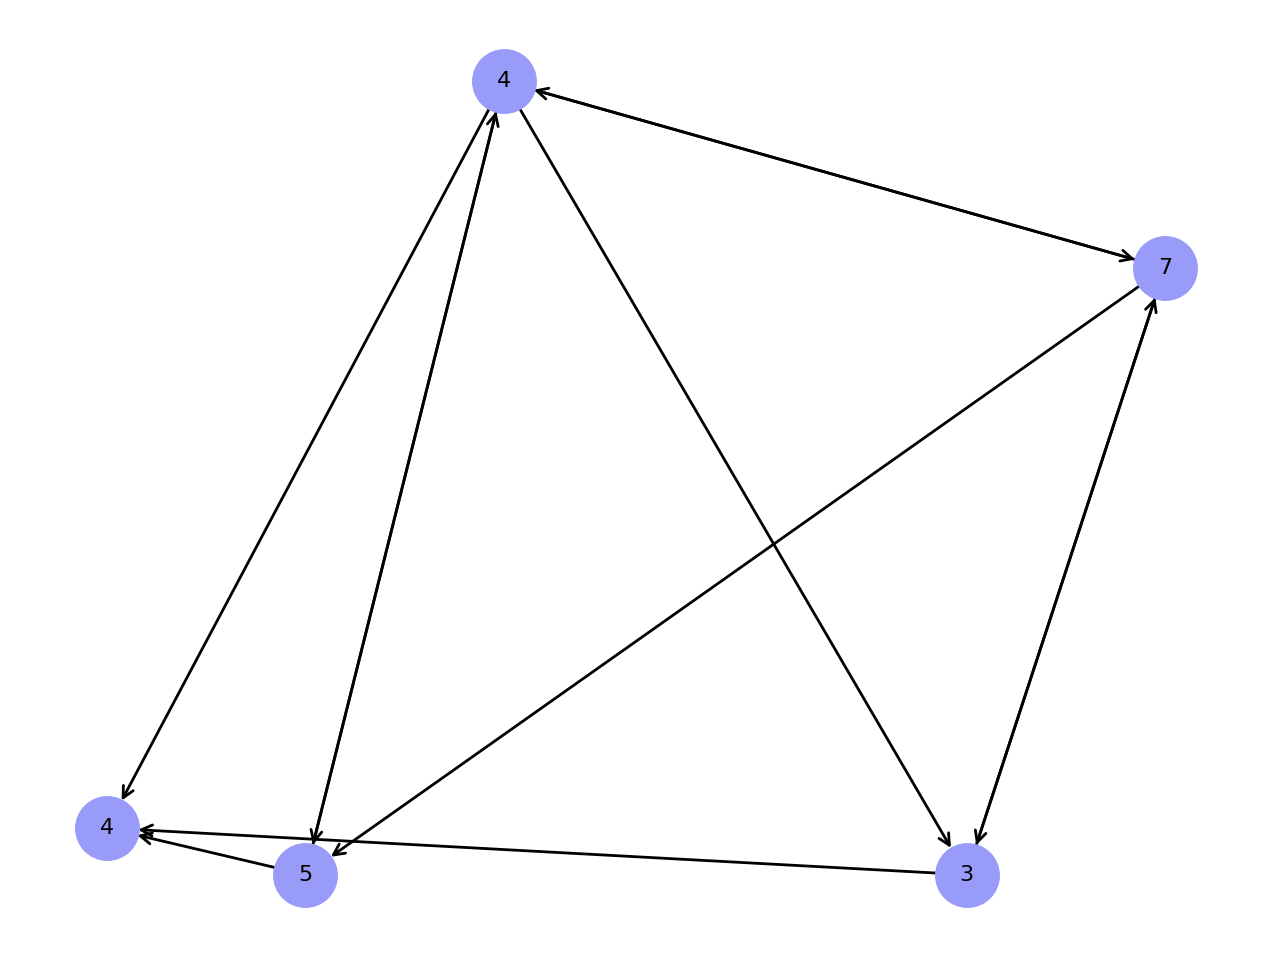
\includegraphics[width=3.65cm]{./figures/random_graph.png} }}%
    \qquad
    \subfloat[\centering With Solution]{{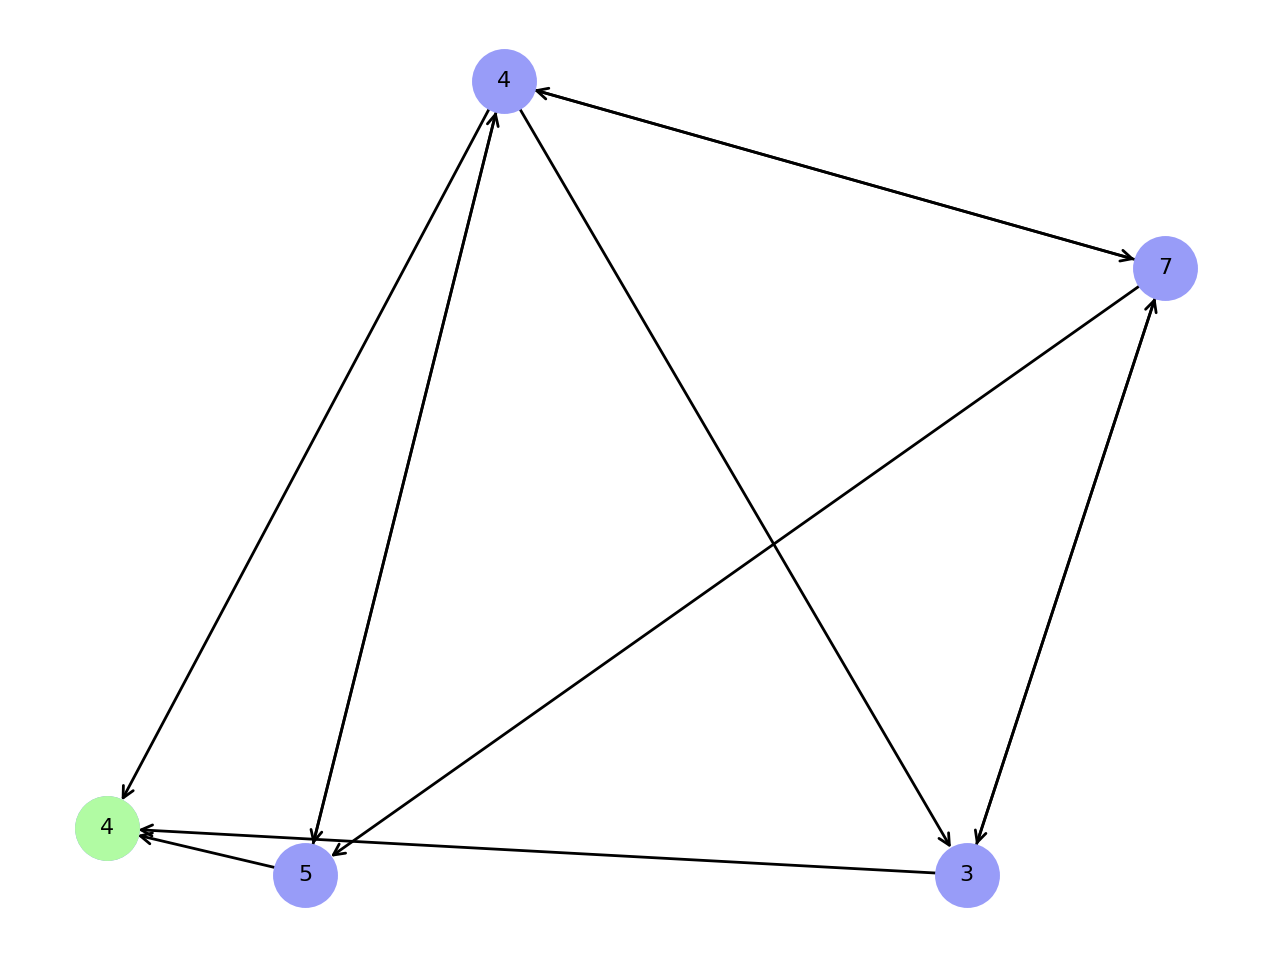
\includegraphics[width=3.65cm]{./figures/random_graph_solution.png} }}%
    \caption{Random Graph and its computed solution}%
    \label{fig:example}%
\end{figure}

% python3 main.py -r 93107 -n 5 -e 0.45

Given this example, and using the \textbf{Exhaustive Search Algorithm}, we first need to compute all the subsets (closures) of the graph, which in this case are 22, and then find the minimum weighted closure, from all candidate solutions, and that can be, as previously mentioned, very inefficient. This can be optimized by passing some parameters that control the algorithm's output. These parameters as well as the algorithm itself will be explained in the following sections.

\section{Implementation Description}

Running the main program, there are a few flags that
can be used.

\begin{figure}[!htb]
    \centering
    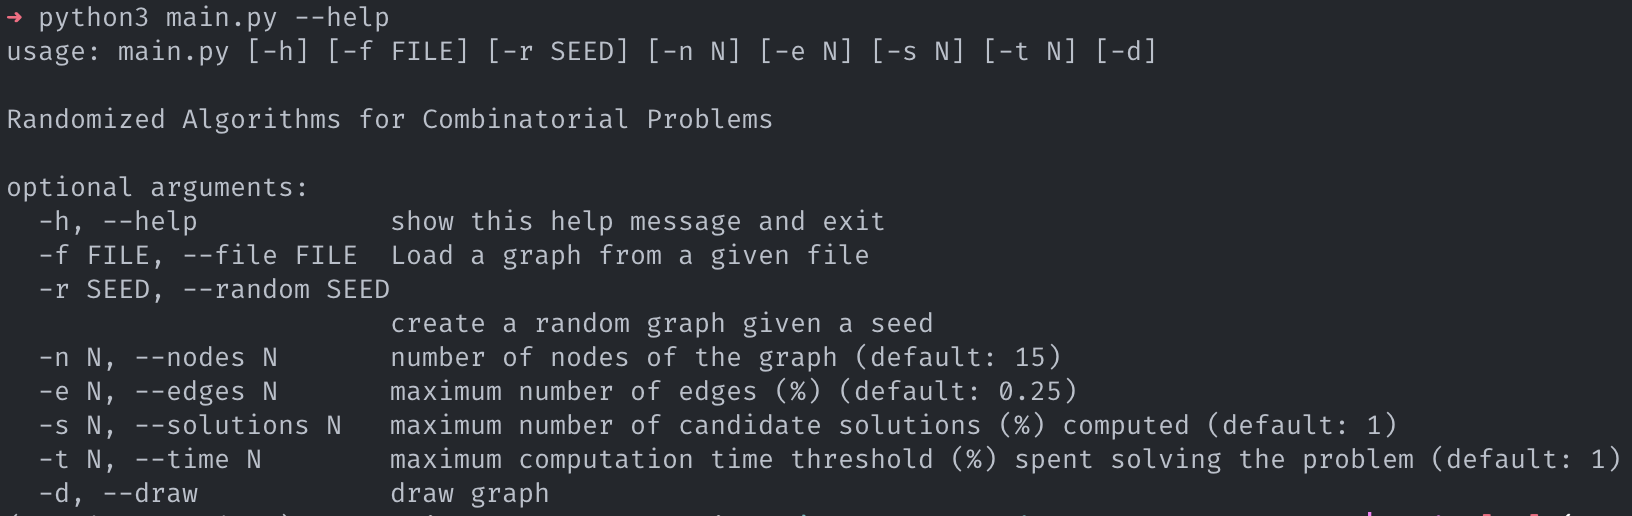
\includegraphics[width=1\columnwidth]{./figures/program_help}
    \caption{Help Menu of the Main Program}
    \label{fig: Help Menu}
\end{figure}

Most of the parameters are the same as in the previous assignment, the ones that are used as part of the randomized algorithm are:
\begin{itemize}
    \item \textbf{-s} - this flag allows the user to define the maximum number of candidate solutions to test, its value belongs in [0, 1], with 1 representing all the possible candidate solutions (100\%) 
    \item \textbf{-i} - this flag allows the user to decide  when  to  stop  testing candidate solutions after spending a certain amount of computation time.
\end{itemize}


\section{Results and Discussion}



\section{Conclusion}

\begin{thebibliography}{9}

\bibitem{networkx}
NetworkX developers. (2014-2022). NetworkX. 
\url{https://networkx.org/}

\bibitem{matplotib}
The Matplotlib development team. (2012-2022). Matplotlib. \url{https://matplotlib.org/}

\bibitem{closure_problem}
GeeksforGeeks. (2022, October 22). Randomized Algorithms. GeeksforGeeks. \url{https://www.geeksforgeeks.org/randomized-algorithms/}

\end{thebibliography}


% use a field named url or \url{} for URLs
% Note: the \bibliographystyle is set automatically

\end{document}
